Esta seção aborda as ferramentas estudadas para compor o ambiente experimental. Cada ferramenta aplica-se à diferentes contextos, tais como: sistema de arquivos distribuídos, gerenciamento de \textit{guests}, servidor web, balanceamento de carga, automação de processos de instalação e testes de carga em bases Cassandra.
\section{Sistema de arquivos distribuídos}
Dentre os principais sistemas de arquivos distribuídos, estudou-se o Ceph e o GlusterFS devido ao fato de possuírem suporte em sistemas Linux e interface POSIX para armazenamento. 

\subsection{Ceph}
    Ceph \cite{Weil2007} é um sistema de arquivos Linux que começou com um projeto de pesquisa na Universidade da Califórnia Santa Cruz (UCSC). É composto por um sistema de arquivos distribuído que incorpora a replicação e a tolerância a falhas, mantendo a compatibilidade POSIX.
    Os objetivos do Ceph podem ser definidos como: fácil escalabilidade para armazenamento de vários petabytes, alto desempenho com cargas de trabalho variáveis e grande confiabilidade \cite{jones}.
    Por meio do Ceph é possível o particionamento dinâmico de metadados e a distribuição e replicação de dados. Também incorpora recursos de tolerância a falhas, presumindo-se que existam falhas em armazenamento em grande escala.
   
   \begin{citacao}
Uma das principais diferenças entre o Ceph e os sistemas de arquivos tradicionais é que, em vez de concentrar a inteligência no sistemas de arquivos em si, a inteligência é distribuída em todo o ecossistema \cite{jones}.
   \end{citacao}

Conforme descrito por \cite{jones}, pode-se definir dois tipos de arquitetura para o Ceph:
    
\subsubsection{Arquitetura conceitual}
\label{subsec:arqconceitual}

    Como ilustra a Figura \ref{fig:arquiteturaceph1}, pode-se dividir o Ceph em 4 módulos: clientes (\textit{clients}), um \textit{cluster} de servidores de metadados (\textit{metadata server cluster}), um \textit{cluster} de armazenamento de objetos (\textit{object storage cluster}) e monitores de cluster (\textit{cluster monitors}).
        
    \begin{figure}[htb]
    \centering
    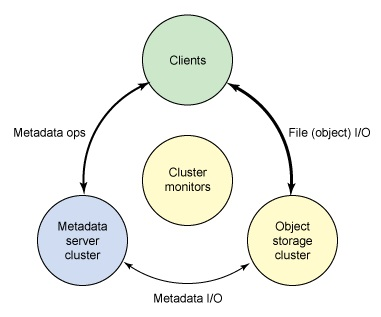
\includegraphics[scale=0.90]{imagens/arquiteturaCeph1.jpg}
    \caption{Arquitetura conceitual do sistema de arquivos distribuídos Ceph} \cite[p. 2]{jones}
    \label{fig:arquiteturaceph1}
    \end{figure}
    
    Os clientes (usuário dos dados) executam operações de metadados, que são operações que localizam os dados utilizando os servidores de metadados. Por esta vez, os servidores de metadados gerenciam a localização de dados já existentes e também de novos dados. E o armazenamento dos metadados é feito no cluster de armazenamento. As funções POSIX como abrir, fechar e renomear, são gerenciadas através dos servidores de metadados, devido aos arquivos de I/O ocorrerem entre o cliente e o \textit{cluster} de armazenamento de objetos. Já as funções POSIX como ler e renomear são gerenciadas diretamente no cluster de armazenamento de objetos \cite{jones}. 
    
\subsubsection{Arquitetura em camadas}
\label{subsec:arqcamadas}

    Conforme a Figura \ref{fig:arquiteturaceph2}, pode-se dividir o Ceph em 3 camadas: interface do cliente (Ceph \textit{client interface}), servidores de metadados (\textit{metadata servers}) e sistema de armazenamento distribuído.
    
    \begin{figure}[htb]
    \centering
    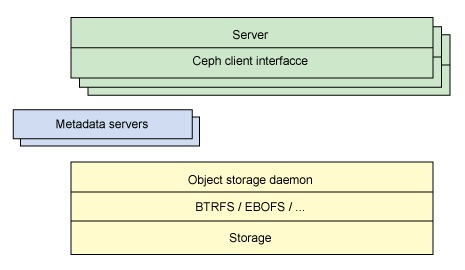
\includegraphics[scale=0.90]{imagens/arquiteturaCeph2.jpg}
    \caption{Arquitetura em camadas do sistema de arquivos distribuídos Ceph} \cite[p. 3]{jones}
    \label{fig:arquiteturaceph2}
    \end{figure}
    
    Na camada de interface, um conjunto de servidores acessa o sistema Ceph através da interface do cliente. Este acesso compreende o relacionamento entre servidores de metadados e armazenamento no nível do objeto. Já na camada de armazenamento distribuído, são projetados o gerenciamento de replicação de dados, a detecção de falhas, a recuperação e a subsequente migração de dados.
    

\subsubsection{Funcionamento}
    A Figura \ref{fig:sistemaceph} exibe a interação dos módulos do projeto Ceph, citados nas arquiteturas \ref{subsec:arqconceitual} e \ref{subsec:arqcamadas}, onde o cliente é o usuário do sistema de arquivos distribuído, o \textit{Ceph metadata daemon} (cmds) fornece os serviços de metadados, o \textit{Ceph object storage daemon} (cosd) fornece o armazenamento real e o \textit{Ceph monitor} (cmon) fornece o gerenciamento de \textit{cluster}. 

    \begin{figure}[htb]
    \centering
    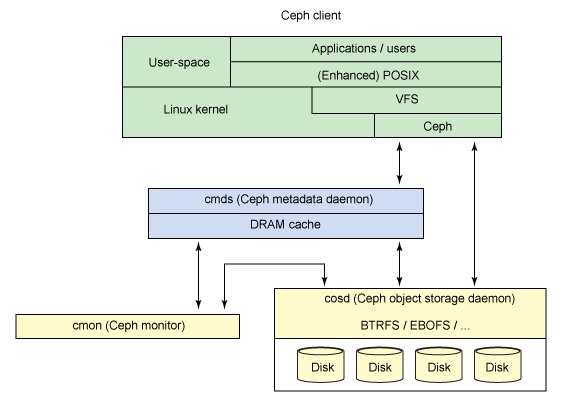
\includegraphics[scale=0.90]{imagens/sistemaCeph.jpg}
    \caption{Funcionamento Sistema Ceph} \cite[p. 4]{jones}
    \label{fig:sistemaceph}
    \end{figure}

Após se conhecer as arquiteturas e a interação entre elas, pode-se destacar as seguintes funcionalidades do Ceph:
\begin{itemize}
 \item Inteligência distribuída:  simplicidade na interface do cliente e capacidade de escalabilidade, mesmo que dinamicamente. Isto se deve ao fato do sistema de arquivos Ceph possuir inteligência distribuída nos nós e não concentrada em um só servidor.
 \item Sistema adaptável: o gerenciamento do espaço de nomes do sistema de arquivos é tarefa do servidor de metadados (cmds). Apesar do armazenamento dos dados ser feito no \textit{cluster} de armazenamento de objetos, o gerenciamento destes é feito separadamente para suportar a escalabilidade. Com isso, o servidor de metadados consegue, de maneira adaptável, replicar e distribuir o espaço de acesso para evitar pontos de acesso.
 \item Tolerância a falhas: quando dispositivos de armazenamento de objetos falham ou novos objetos são adicionados, monitores detectam e mantêm um mapa de cluster válido mesmo que de modo distribuído. 
 \end{itemize}


 
\subsection{GlusterFS}
\label{sec:gluster}

GlusterFS é um sistema de arquivos distribuídos e descentralizado, de código aberto, com escalabilidade a nível de petabytes e com conexões de milhares de clientes, criado recentemente e ainda em desenvolvimento pela empresa Z Research. É um sistema de arquivos com um \textit{design} modular, empilhável e sua arquitetura eliminou a localização de metadados através da utilização do algoritmo de hash elástico (\textit{Hashing Algorithm Elastic} \footnote{O algoritmo de hash elástico é utilizado para localizar dados no conjunto de armazenamento, remover gargalos de I/O e eliminiar pontos de falha. O acesso aos dados é totalmente paralelizado e o desempenho é linearmente escalável.}). Tal arquitetura garante melhor desempenho, escalabilidade linear e confiabilidade. O objetivo principal deste sistema é a escalabilidade, sendo que para isso seus projetistas utilizaram conceitos da computação de alto desempenho, como a agregação. Sobre ele, pode-se executar diversos sistemas operacionais, como Linux, FreeBSD, OpenSolaris e Mac OS X \cite{Mohanty2014} .

Basicamente, GlusterFS agrega múltiplas unidades de armazenamento remotas em um único volume. As unidades de armazenamento, chamadas \textit{bricks}, são distribuídas pela rede em um único sistema de arquivos paralelo, permitindo uma escalabilidade de milhares de \textit{bricks} e vários petabytes de armazenamento. Os clientes, que também podem ser simultaneamente servidores de dados, montam os diretórios compartilhados pelos servidores, tendo assim acesso a uma parte ou a todo o conteúdo compartilhado.

A maior parte das funcionalidades no GlusterFS são implementadas através de tradutores, que são objetos binários compartilhados, carregados em tempo de execução. Esses objetos possuem interfaces de comunicação estritamente definidas, de modo que os mesmos podem ser carregados tanto pelos clientes como pelos servidores. O conceito de tradutores foi herdado do sistema operacional GNU Hurd. Novos tradutores podem ser escritos através de uma interface definida pelo GlusterFS. Toda a implementação do sistema é feita no espaço de usuário do sistema operacional, através do módulo Fuse (\textit{Filesystem in Userspace}). Isso proporciona maior flexibilidade ao administrador, que não precisa ter privilégios especiais para carregar o sistema. Porém, o desempenho pode ser afetado, uma vez que se faz necessário um elevado número de cópias da memória do espaço de usuário para o espaço do núcleo do sistema operacional.

Os servidores GlusterFS são compatíveis com POSIX, desta forma, é possível utilizar qualquer sistema de arquivos \textit{ondisk} que suporta atributos estendidos (ext4, XFS, entre outros) para formatar e para armazenar dados em discos. O acesso aos dados pode ser feito utilizando protocolos de acesso padrão da indústria, como \textit{Network File System} (NFS) e \textit{Servidor Message Block} (SMB).

O sistema GlusterFS consiste em vários nós interligados, formando um \textit{cluster} para organizar e manipular grandes quantidades de arquivos e permitir que aplicações consigam utilizar este recurso. Conforme a Figura \ref{fig:glusterArq}, o modelo de comunicação utilizado por este sistema de arquivos é o Mestre/Escravo.

    \begin{figure}[htb]
    \centering
    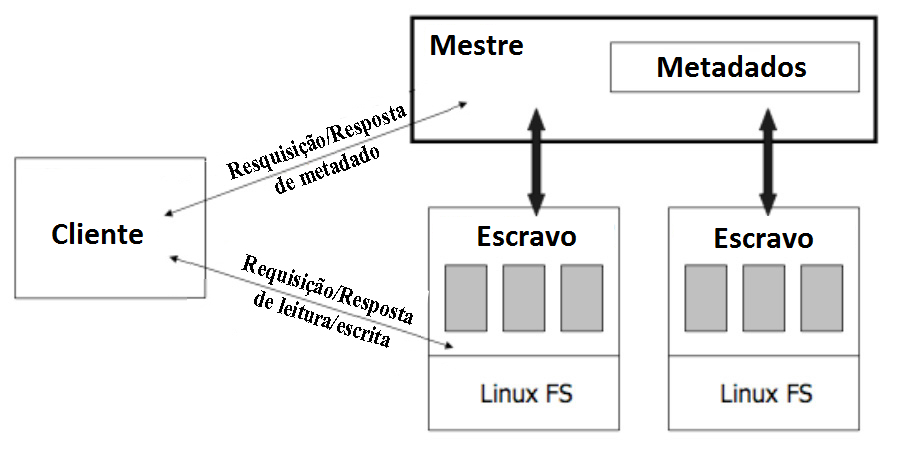
\includegraphics[scale=0.50]{imagens/GlusterFSArq.png}
    \caption{Arquitetura do GlusterFS} \cite{Roman2012}
    \label{fig:glusterArq}
    \end{figure}    

O Mestre é o responsável por coordenar o \textit{cluster}. Ele informa ao cliente a localização de cada fragmento que compõe o arquivo. Tais fragmentos ficam armazenados nos Escravos e possuem tamanho de 64 MB. 


\section{Gerenciador de \textit{Guests}}

Existem várias ferramentas de virtualização como: Virtualbox, VMWare, Xen, Virt-Manager, entre outras. O Virt-Manager foi escolhido como objeto de estudo por ser \textit{Open Source} e por possuir o KVM como módulo de virtualização, o qual já está incluído nas distribuições Linux.

\subsection{Virt-Manager}

Virt-Manager é uma interface gráfica que possui diversos software em camadas abaixo da interface gráfica, que são responsáveis pela flexibilidade do Virt-Manager \cite{PabloHess}.

    A primeira camada é composta pelo libvirt, uma API que oferece uma forma unificada de executar ações em múltiplas plataformas de virtualização, o qual suporta as seguintes plataformas: KVM, QEMU, Xen, VirtualBox, VMware, entre outras \cite{libvirt}.

    A segunda camada tratará sobre o KVM (\textit{Kernel-based Virtual Machine}).
    
    \subsection{KVM}
   KVM é um módulo que provê a pilha de software necessária para virtualização \cite{kvm}. Ele é um software de código aberto que permite a criação de \textit{guests} e também é visto como um subsistema do Linux, uma vez que seu componente de \textit{kernel} está incluído nas distribuições Linux (a partir da versão 2.6.20). Quando utilizado com QEMU (Quick EMUlator) permite a criação de uma \textit{guest} que executa com baixo \textit{overhead} (sistema criado na \textit{guest} funciona semelhante ao que roda na máquina física) \cite{KVM2}.
    As principais características do KVM são: gerenciamento de \textit{guests} com segurança, substituição de várias máquinas físicas por um servidor virtual, auxiliando assim o desenvolvimento de novos sistemas.

    
    \begin{figure}[htb]
    \centering
    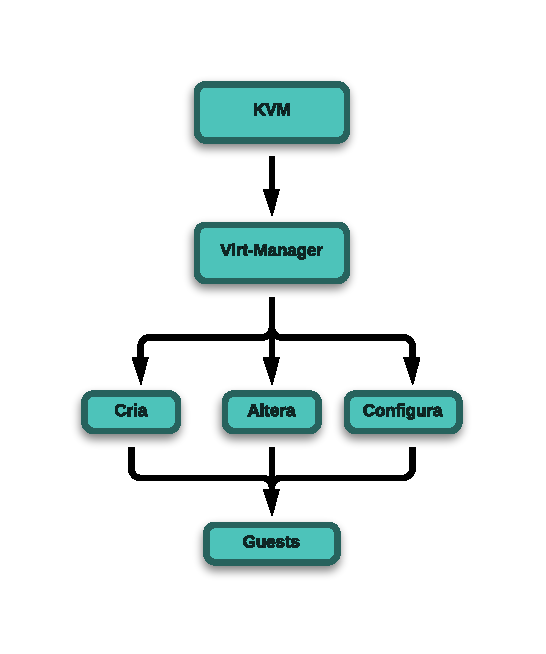
\includegraphics[scale=0.80]{imagens/kvm.pdf}
    \caption{Diagrama KVM x \textit{Virt-Manager}}
    \label{fig:kvm}
    \end{figure} 
    
    A Figura \ref{fig:kvm} exibe o diagrama \textit{botton-up} do sistema de gerenciamento de \textit{guests}. O sistema de virtualização do KVM conta com um sistema de gerenciamento chamado de Virt-manager, que provê um ambiente gráfico através do qual se pode criar, configurar e alterar os parâmetros da máquina virtual, incluindo os recursos de memória, configurações de rede e disco \cite{KVM2}.


\section{Balanceamento de Carga}

    O balanceamento de carga é um método utilizado para a distribuição de cargas de trabalho entre recursos de computação, tais como computadores, \textit{cluster} de computadores, ligações de rede, unidades de processamento central ou unidades de disco. O balanceamento de carga tem como objetivo otimizar a utilização de recursos, maximizar a produção, minimizar o tempo de resposta e evitar a sobrecarga de qualquer um dos recursos. Utilizando múltiplos componentes com o balanceamento de carga, em vez de um único componente pode-se aumentar a confiabilidade através da redundância. O balanceamento de carga é normalmente fornecido pelo software ou hardware dedicado, como um switch multicamada ou um processo do servidor DNS.

    O balanceamento consiste principalmente em reencaminhar o tráfego por caminhos alternativos a fim de descongestionar os servidores mais sobrecarregados.

\subsection{Nginx}

O Nginx é um servidor web com balanceamento de carga escrito por Igor Sysoev. O projeto surgiu em 2002 para atender as necessidades de um site russo com alto tráfego, cerca de 500 milhões de requisições por dia. Hoje o sistema é utilizado por diversos sites, tais como: SourceForge e Hulu.com. Ele trabalha com grande volume de requisições HTTP e torna as aplicações web mais ágeis, escaláveis, rápidas e seguras \cite{nginx}.

Dentre as principais características deste servidor web, estão:

\begin{itemize}
\item Velocidade: o servidor Nginx faz o uso de soquetes assíncronos. Um processo por núcleo é o suficiente para atender milhares de conexões, diminuindo a carga da CPU e o consumo de memória.
\item Facilidade de uso: suas configurações são mais simples de serem ajustadas que outros servidores web, como Apache. Em poucas linhas é possível configurar o servidor. 
\item Modularidade:  Nginx além de possuir código aberto, possui diversos \textit{plug-in} que atuam como módulos para as mais variadas funcionalidades.
\end{itemize}



A Figura \ref{fig:nginx}, exibe a arquitetura modular do Nginx. Ele é composto por núcleo e módulos funcionais. O núcleo é responsável por manter a conexão entre os diferentes módulos nas diferentes etapas de processamento, funcionamento este conhecido como Mestre/Escravo. A arquitetura modular permite aos desenvolvedores estender o conjunto de recursos do servidor web sem modificar o núcleo, sendo esta uma das principais vantagens do Nginx.

    \begin{figure}[htb]
    \centering
    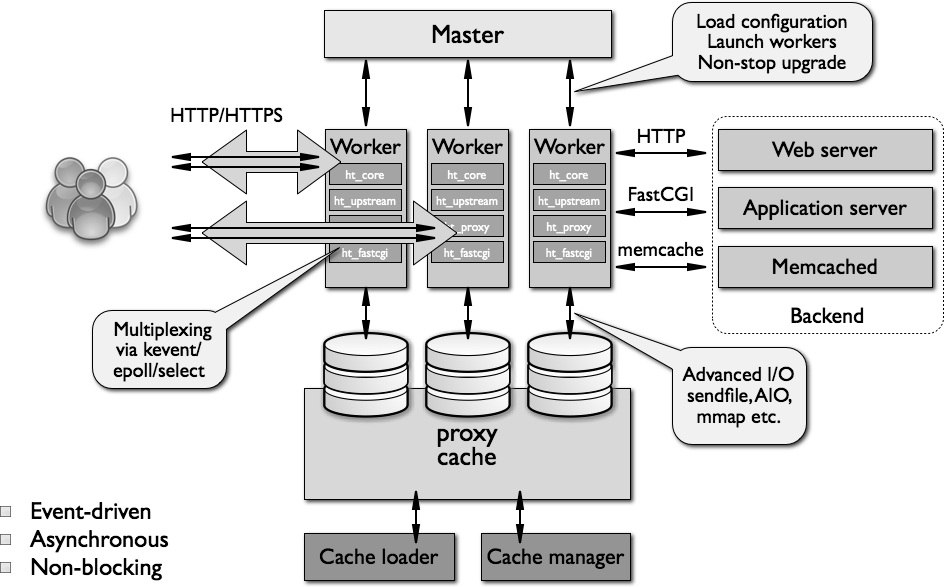
\includegraphics[scale=0.40]{imagens/nginx.png}
    \caption{Arquitetura do Nginx} \cite{nginx}
    \label{fig:nginx}
    \end{figure} 

O Nginx é comumente instalado entre a rede e a aplicação para gerenciar o processamento de concorrência, o endereçamento de URL, o balanceamento de carga HTTP, terminação SSL, cache e políticas de segurança. O serviço de balanceamento de carga e cache de conteúdo visam oferecer uma plataforma rentável e altamente disponível para os aplicativos hospedados. O balanceamento de carga é feito a partir das requisições recebidas pelo \textit{frontend} e distribuidas entre os \textit{backends} (servidores de aplicativos). Ele fornece balanceamento de dois níveis com base em cookies. O primeiro é à uma taxa de um nó. E o segundo é à velocidade de um grupo de nós interligados por uma mesma sessão \cite{Jelastic2014}.


\subsection{HAProxy}

O HAProxy é um balanceador de carga de alto desempenho para HTTP e TCP. Ele recebe as conexões dos usuários e atua como um \textit{proxy}, criando um canal entre o usuário e um dos servidores de aplicação. De acordo com \textit{benchmarks} elaborados pelo desenvolvedor, a ferramenta possui desempenho de mais de 40 mil conexões por segundo utilizando rede de 10 Gbps \cite{HAProxy2009}.

Esta aplicação possui alguns mecanismos para escolher o servidor web que deve encaminhar a solicitação ao usuário. Dentre as estratégias de escalonamento suportadas, estão:

\begin{itemize}
\item \textit{Round-robin}: o servidor é escolhido de forma circular, independente da carga em cada um dos servidores de aplicação;
\item Menos conexões: o servidor com menos conexões é escolhido, o que garante que o servidor mais ocioso seja utilizado;
\item Cookie: o HAProxy tentará sempre indicar o mesmo servidor que o usuário conectou pela primeira vez e
\item Hash de IP: neste caso a aplicação irá escolher o servidor de acordo com o IP.
\end{itemize}

\section{Kickstart - Fedora}

Kickstart é um sistema utilizado para automatizar processos de instalações, parcialmente ou em sua totalidade. Os arquivos são configurados para conter as respostas para as perguntas feitas pelos programas de instalação, tais como fuso horário, unidade que deve ser particionada, nome do sistema, nome dos usuários, quais pacotes devem ser instalados, entre outras. Os arquivos Kickstart geralmente são utilizados para implantar o SO em um grande número de máquinas de uma só vez, sem que haja intervenção humana no processo \cite{Fedora}.

\subsection{Utilizando o Kickstart}

As instalações Kickstart podem ser realizadas utilizando um DVD local, um disco rígido local, ou através do NFS, FTP, HTTP, ou HTTPS.

Para utilizar o Kickstart deve-se:
\begin{itemize}
\item criar um arquivo Kickstart;
\item criar uma mídia de inicialização ou configurar um servidor de inicialização de rede (PXE);
\item disponibilizar o arquivo Kickstart em uma mídia removível, ou em uma unidade de disco rígido, ou em um local de rede e
\item na opções de \textit{boot}, informar ao instalador onde encontrar o arquivo Kickstart.
\end{itemize}




    \begin{figure}[htb]
    \centering
    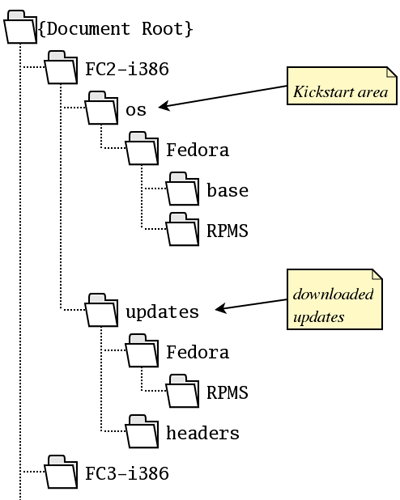
\includegraphics[scale=0.60]{imagens/kickstart.png}
    \caption{Estrutura de um diretório de repositório \textit{yum}, hospedado em servidor KickStart} \cite{McCallum2005}
    \label{fig:kickstartdir}
    \end{figure} 





\section{JMeter}

O JMeter é uma ferramenta \textit{desktop} para testes de desempenho, desenvolvida utilizando a linguagem Java e licenciada sob os termos da Licença Apache, versão 2.0. Esta ferramenta foi primeiramente utilizada para realizar testes em aplicações web, mas tem expandido suas funcionalidades, podendo realizar testes funcionais em bancos de dados \cite{De2013}.

Como o JMeter é totalmente desenvolvido em Java, é possível operá-lo em qualquer sistema operacional que possua Java instalado.

\subsection{CassJMeter}
\label{sec:cassjmeter}

O CassJMeter é um \textit{plugin} que foi desenvolvido pela Netflix para realizar testes de carga em banco de dados Cassandra. Ele funciona como um cliente de Cassandra e pode enviar requisições utilizando as interfaces Astyanax ou Thrift \cite{DenisSheahan2012}.

De acordo com o estudo de caso realizado pela Netflix, usando 60 instâncias adicionais como clientes e executando o programa de estresse (CassJMeter) conseguiu-se atender a uma carga de trabalho de 1,1 milhões de clientes escrevendo por segundo. Os dados foram automaticamente replicadas em três zonas, perfazendo um total de 3,3 milhões de gravações por segundo em todo o \textit{cluster} \cite{Crockcroft2011}. 
Para medir a escalabilidade, o mesmo teste foi executado com 48, 96, 144 e 288 casos, com respectivamente 10, 20, 30 e 60 clientes. A carga sobre cada instância foi muito semelhante em todos os casos, conforme mostra a Figura \ref{fig:benchNetflix}.

    \begin{figure}[htb]
    \centering
    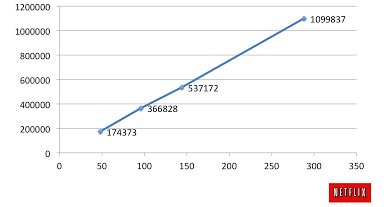
\includegraphics[scale=0.7]{imagens/scale.png}
    \caption{Escalabilidade linear do \textit{cluster} Cassandra com fator de replicação 3} \cite{Crockcroft2011}
    \label{fig:benchNetflix}
    \end{figure} 

\section{Base de dados (Cassandra)}

O Cassandra é um sistema de banco de dados NoSQL. Ele é um banco de dados altamente escalável, capaz de gerenciar grandes volumes de dados em vários \textit{datacenters} e em nuvem. Este banco também oferece disponibilidade contínua, escalabilidade linear, modelo dinâmico de dados e tempos de respostas rápidos.

Estas e outras características, bem como o porquê da escolha desssa base de dados serão melhor estudadas no Capítulo \ref{cap:cassandra}. 